% ==== Document Class & Packages =====
\documentclass[12pt,hidelinks]{article}
    \usepackage[european,straightvoltages]{circuitikz}
	\usepackage[explicit]{titlesec}
	\usepackage{titletoc}
    \usepackage{amsmath}
    \usepackage{amssymb}
    \usepackage{arydshln}
    \usepackage{changepage}
    \usepackage{multirow}
	\usepackage{tocloft}
	\usepackage{charter}
	\usepackage[many]{tcolorbox}
	\usepackage{amsmath}
	\usepackage{graphicx}
	\usepackage{xcolor}
	\usepackage{tikz,lipsum,lmodern}
	\usetikzlibrary{calc}
	\usepackage[english]{babel}
	\usepackage{fancyhdr}
	\usepackage{mathrsfs}
	\usepackage{empheq}
	\usepackage{fourier}% change to lmodern if fourier is no available
	\usepackage{wrapfig}
	\usepackage{fancyref}
	\usepackage{hyperref}
	\usepackage{cleveref}
	\usepackage{listings}
	\usepackage{varwidth}
	\usepackage{longfbox}
	\usepackage{geometry}
    \usepackage{ragged2e}
	\usepackage{marginnote}
	\tcbuselibrary{theorems}
	\tcbuselibrary{breakable, skins}
	\tcbuselibrary{listings, documentation}
	\geometry{
		a4paper,
		left=33mm,
		right=33mm,
		top=20mm}
% ========= Path to images ============
%   - Direct the computer on the path 
% 	  to the folder containg the images
% =====================================
\graphicspath{{./images/}}
% ============= Macros ================
\newcommand{\ubar}[1]{\text{\b{$#1$}}}
\newcommand{\fillin}{\underline{\hspace{.75in}}{\;}}
\newcommand{\solution}{\textcolor{mordantred19}{Solution:}}
\setlength{\parindent}{0pt}
\addto{\captionsenglish}{\renewcommand*{\contentsname}{Table of Contents}}
\linespread{1.2}
% ======== Footers & Headers ==========
\cfoot{\thepage}
\chead{}\rhead{}\lhead{}
% =====================================
\renewcommand{\thesection}{\arabic{section}}
\newcommand\sectionnumfont{% font specification for the number
	\fontsize{114}{39}\color{myblueii}\selectfont}
\newcommand\sectionnamefont{% font specification for the name "PART"
	\normalfont\color{white}\scshape\small\bfseries }
% ============= Colors ================
% ----- Red -----
\definecolor{mordantred19}{rgb}{0.68, 0.05, 0.0}
% ----- Blue -----
\definecolor{st.patrick\'sblue}{rgb}{0.14, 0.16, 0.48}
\definecolor{teal}{rgb}{0.0, 0.5, 0.5}
\definecolor{beaublue}{rgb}{0.74, 0.83, 0.9}
\definecolor{mybluei}{RGB}{0,173,239}
\definecolor{myblueii}{RGB}{63,200,244}
\definecolor{myblueiii}{RGB}{199,234,253}
% ---- Yellow ----
\definecolor{blond}{rgb}{0.98, 0.94, 0.75}
\definecolor{cream}{rgb}{1.0, 0.99, 0.82}
% ----- Green ------
\definecolor{emerald}{rgb}{0.31, 0.78, 0.47}
\definecolor{darkspringgreen}{rgb}{0.09, 0.45, 0.27}
% ---- White -----
\definecolor{ghostwhite}{rgb}{0.97, 0.97, 1.0}
\definecolor{splashedwhite}{rgb}{1.0, 0.99, 1.0}
% ---- Grey -----
\definecolor{whitesmoke}{rgb}{0.96, 0.96, 0.96}
\definecolor{lightgray}{rgb}{0.92, 0.92, 0.92}
\definecolor{floralwhite}{rgb}{1.0, 0.98, 0.94}
% ========= Part Format ==========
\titleformat{\section}
{\normalfont\huge\filleft}
{}
{20pt}
{\begin{tikzpicture}[remember picture,overlay]
	\fill[myblueiii] 
	(current page.north west) rectangle ([yshift=-6cm]current page.north east);   
\node[
	fill=mybluei,
	text width=2\paperwidth,
	rounded corners=3cm,
	text depth=6cm,
	anchor=center,
	inner sep=0pt] at (current page.north east) (parttop)
	{\thepart};%
\node[
	anchor=south east,
	inner sep=0pt,
	outer sep=0pt] (partnum) at ([xshift=-20pt]parttop.south) 
	{\sectionnumfont\thesection};
\node[
	anchor=south,
	inner sep=0pt] (partname) at ([yshift=2pt]partnum.south)   
	{\sectionnamefont SECTION};
\node[
	anchor=north east,
	align=right,
	inner xsep=0pt] at ([yshift=-0.5cm]partname.east|-partnum.south) 
	{\parbox{.7\textwidth}{\raggedleft#1}};
\end{tikzpicture}%
}
% ========= Hyper Ref ===========
\hypersetup{
	colorlinks,
	linkcolor={red!50!black},
	citecolor={blue!50!black},
	urlcolor={blue!80!black}
}
% ========= Example Boxes =============
\tcbset{
	defstyle/.style={
		fonttitle=\bfseries\upshape, 
		fontupper=\slshape,
		arc=0mm, 
		beamer,
		colback=blue!5!white,
		colframe=blue!75!black},
	theostyle/.style={
		fonttitle=\bfseries\upshape, 
		fontupper=\slshape,
		colback=red!10!white,
		colframe=red!75!black},
	visualstyle/.style={
		height=6.5cm,
		breakable,
		enhanced,
		leftrule=0pt,
		rightrule=0pt,
		bottomrule=0pt,
		outer arc=0pt,
		arc=0pt,
		colframe=mordantred19,
		colback=lightgray,
		attach boxed title to top left,
		boxed title style={
			colback=mordantred19,
			outer arc=0pt,
			arc=0pt,
			top=3pt,
			bottom=3pt,
		},
		fonttitle=\sffamily,},
	discussionstyle/.style={
		height=6.5cm,
		breakable,
		enhanced,
		rightrule=0pt,
		toprule=0pt,
		outer arc=0pt,
		arc=0pt,
		colframe=mordantred19,
		colback=lightgray,
		attach boxed title to top left,
		boxed title style={
			colback=mordantred19,
			outer arc=0pt,
			arc=0pt,
			top=3pt,
			bottom=3pt,
		},
		fonttitle=\sffamily},
	mystyle/.style={
		height=6.5cm,
		breakable,
		enhanced,
		rightrule=0pt,
		leftrule=0pt,
		bottomrule=0pt,
		outer arc=0pt,
		arc=0pt,
		colframe=mordantred19,
		colback=lightgray,
		attach boxed title to top left,
		boxed title style={
			colback=mordantred19,
			outer arc=0pt,
			arc=0pt,
			top=3pt,
			bottom=3pt,
		},
		fonttitle=\sffamily},
	aastyle/.style={
			height=3.5cm,
			enhanced,
			colframe=teal,
			colback=lightgray,
			colbacktitle=floralwhite,
			fonttitle=\bfseries,
			coltitle=black,
		attach boxed title to top center={
	  		yshift=-0.25mm-\tcboxedtitleheight/2,
	   		yshifttext=2mm-\tcboxedtitleheight/2}, 
		boxed title style={boxrule=0.5mm,
			frame code={ \path[tcb fill frame] ([xshift=-4mm]frame.west)
				-- (frame.north west) -- (frame.north east) -- ([xshift=4mm]frame.east)
				-- (frame.south east) -- (frame.south west) -- cycle; },
			interior code={ 
				\path[tcb fill interior] ([xshift=-2mm]interior.west)
				-- (interior.north west) -- (interior.north east)
				-- ([xshift=2mm]interior.east) -- (interior.south east) -- (interior.south west)
				-- cycle;} }
				},
	examstyle/.style={
		height=9.5cm,
		breakable,
		enhanced,
		rightrule=0pt,
		leftrule=0pt,
		bottomrule=0pt,
		outer arc=0pt,
		arc=0pt,
		colframe=mordantred19,
		colback=lightgray,
		attach boxed title to top left,
		boxed title style={
			colback=mordantred19,
			outer arc=0pt,
			arc=0pt,
			top=3pt,
			bottom=3pt,
		},
		fonttitle=\sffamily},
	doc head command={
		interior style={
			fill,
			left color=yellow!20!white, 
			right color=white}},
	doc head environment={
		boxsep=4pt,
		arc=2pt,
		colback=yellow!30!white,
		},
	doclang/environment content=text
}
% ============= Boxes ================
\newtcolorbox[auto counter,number within=section]{example}[1][]{
	mystyle,
	title=Example~\thetcbcounter,
	overlay unbroken and first={
		\path
		let
		\p1=(title.north east),
		\p2=(frame.north east)
		in
		node[anchor=
			west,
			font=\sffamily,
			color=st.patrick\'sblue,
			text width=\x2-\x1] 
		at (title.east) {#1};
	}
}
\newtcolorbox[auto counter,number within=section]{longexample}[1][]{
	examstyle,
	title=Example~\thetcbcounter,
	overlay unbroken and first={
		\path
		let
		\p1=(title.north east),
		\p2=(frame.north east)
		in
		node[anchor=
		west,
		font=\sffamily,
		color=st.patrick\'sblue,
		text width=\x2-\x1] 
		at (title.east) {#1};
	}
}
\newtcolorbox[auto counter,number within=section]{example2}[1][]{
	aastyle,
	title=Example~\thetcbcounter,{}
}
\newtcolorbox[auto counter,number within=section]{discussion}[1][]{
	discussionstyle,
	title=Discussion~\thetcbcounter,
	overlay unbroken and first={
		\path
		let
		\p1=(title.north east),
		\p2=(frame.north east)
		in
		node[anchor=
		west,
		font=\sffamily,
		color=st.patrick\'sblue,
		text width=\x2-\x1] 
		at (title.east) {#1};
	}
}
\newtcolorbox[auto counter,number within=section]{visualization}[1][]{
	visualstyle,
	title=Visualization~\thetcbcounter,
	overlay unbroken and first={
		\path
		let
		\p1=(title.north east),
		\p2=(frame.north east)
		in
		node[anchor=
		west,
		font=\sffamily,
		color=st.patrick\'sblue,
		text width=\x2-\x1] 
		at (title.east) {#1};
	}
}
% --------- Theorems ---------
\newtcbtheorem[number within=subsection,crefname={definition}{definitions}]%
	{Definition}{Definition}{defstyle}{def}%
\newtcbtheorem[use counter from=Definition,crefname={theorem}{theorems}]%
	{Theorem}{Theorem}{theostyle}{theo}
	%
\newtcbtheorem[use counter from=Definition]{theo}{Theorem}%
{
	theorem style=plain,
	enhanced,
	colframe=blue!50!black,
	colback=yellow!20!white,
	coltitle=red!50!black,
	fonttitle=\upshape\bfseries,
	fontupper=\itshape,
	drop fuzzy shadow=blue!50!black!50!white,
	boxrule=0.4pt}{theo}
\newtcbtheorem[use counter from=Definition]{DashedDefinition}{Definition}%
 {
 	enhanced,
 	frame empty,
 	interior empty,
 	colframe=darkspringgreen!50!white,
	coltitle=darkspringgreen!50!black,
	fonttitle=\bfseries,
	colbacktitle=darkspringgreen!15!white,
	borderline={0.5mm}{0mm}{darkspringgreen!15!white},
	borderline={0.5mm}{0mm}{darkspringgreen!50!white,dashed},
	attach boxed title to top center={yshift=-2mm},
	boxed title style={boxrule=0.4pt},
	varwidth boxed title}{theo}
%%%%%%%%%%%%%%%%%%%%%%%%%%%%%%%%%%%%%%%%
\newtcblisting[auto counter,number within=section]{disexam}{
	skin=bicolor,
	colback=white!30!beaublue,
	colbacklower=white,
	colframe=black,
	before skip=\medskipamount,
	after skip=\medskipamount,
	fontlower=\footnotesize,
	listing options={style=tcblatex,texcsstyle=*\color{red!70!black}},}
%%%%%%%%%%%%%%%%%%%%%%%%%%%%%%%%%%%%%%%

\begin{document}
\begin{titlepage}
	\centering % Center everything on the title page
	\scshape % Use small caps for all text on the title page
	\vspace*{1.5\baselineskip} % White space at the top of the page
% ===================
%	Title Section 	
% ===================

	\rule{13cm}{1.6pt}\vspace*{-\baselineskip}\vspace*{2pt} % Thick horizontal rule
	\rule{13cm}{0.4pt} % Thin horizontal rule
	
		\vspace{0.75\baselineskip} % Whitespace above the title
% ========== Title ===============	
	{	\Huge Fiches de Physiques\\ 
			\vspace{4mm}
		   PTSI \\	}
% ======================================
		\vspace{0.75\baselineskip} % Whitespace below the title
	\rule{13cm}{0.4pt}\vspace*{-\baselineskip}\vspace{3.2pt} % Thin horizontal rule
	\rule{13cm}{1.6pt} % Thick horizontal rule
	
		\vspace{1.75\baselineskip} % Whitespace after the title block
% =================
%	Information	
% =================
	{\large Noë Charlier \\
		\vspace*{1.2\baselineskip}
	2021-2022} \\
	\vfill
\end{titlepage}
%%%%%%%%%%%%%%%%%%%%%%%%%%%%%%%%%%%%%%%%%%%%%%%%%%%%%%%%%%%
\tableofcontents
\vfill
\small{\noindent \textbf{À propos} \vspace{-3mm}\\
\noindent \rule{3.3cm}{0.5pt} \\
Le but est de produire des courtes fiches pour réviser facilement les concours.\\
L'intégralité du contenu de ce fichier et de ce dossier est gratuite pour un usage public.}
\newpage
\newgeometry{
	left=29mm, 
	right=29mm, 
	top=20mm, 
	bottom=15mm}
%%%%%%%%%%%%%%%%%%%%%%%%%%%%%%%%%%%%%%%%%%%%%%%%%%%%%%%%%%%
\section{Analyse Dimensionnelle}
\vspace{3cm}
	L'analyse dimensionnelle est essentiel en physique, elle permet de vérifier l'homogénéité !
	\subsection{Tableau récapitulatif}
			\begin{table}[h!]
            \centering
            \begin{tabular}{c|c|c}
            Grandeur & Unité SI & Dimension \\\hline
            Longueur & mètre(m) & L  \\
            Masse & kilogramme(kg) & M  \\
            Durée & seconde(s) & T  \\
            Température & kelvin(K) & $\theta$ \\
            Intensité éclectique & ampère(A) & I \\
            Quantité de matière & mole(mol) & N\\
            Intensité lumineuse & candela(Cd) & J
            \end{tabular}
            \caption{\label{tab:table1}Unité du Système International (USI)}
            \label{table:1}
            \end{table}
\newpage
%%%%%%%%%%%%%%%%%%%%%%%%%%%%%%%%%%%%%%%%%%%%%%%%%%%%%%%%%%%
\section{Fondements de l'optique géométrique}
\vspace{3cm}
    Loi de Snell Descartes, Spectres d’émission, Indice optique...
    \subsection{Milieu d'étude} 
         On s’intéressera à la propagation de la lumière dans des milieux qualifiés de \textbf{Transparents, Linéaires, Homogènes et Isotropes.}
         \subsubsection{Indice de réfraction}
            \[n=\frac{c}{v}\]
            Avec: $n$ l'indice, $c$ la célérité, et $v$ la vitesse dans le milieu.
    \subsection{Lois de Snell-Descartes}
        \begin{DashedDefinition}{}[
        \begin{itemize}
            \item Rayon réflechi et réfracté sur le même plan d'incidence.
            \item Le rayon est symétrique par rapport à la normal au dioptre.
            \item Le rayon réfracté vérifie: \fbox{$n_1 sin(i_1) = n_2 sin (i_2)$}
        \end{itemize}
        \end{DashedDefinition}
\newpage
%%%%%%%%%%%%%%%%%%%%%%%%%%%%%%%%%%%%%%%%%%%%%%%%%%%%%%%%%%%
\section{Systèmes optiques usuels}
\vspace{3cm}
Lentille mince convergente/divergente, distance focale, relation de conjugaison.
    \subsection{Grandissement}
        Le grandissement transversal est le rapport entre la taille de l'image et celle de l'objet:
        \[ \gamma = \frac{\overline{A'B'}}{\overline{AB}}\]
	\subsection{Conditions de Gauss} 
        \begin{DashedDefinition}{}[
        \begin{itemize}
            \item Le rayon est proche de l'axe optique.
            \item Le rayon est peu inclé par rapport à l'axe optique.
        \end{itemize}
        Les rayons sont \textbf{paraxiaux}
        \end{DashedDefinition}
	\subsection{Modèle de l'oeil}
        \begin{itemize}
            \item Le \textbf{cristallin} est la lentille.
            \item la \textbf{pupille} est le diaphragme.
            \item la \textbf{rétine} est l'écran.
        \end{itemize}
        Limite de \textbf{résolution angulaire pour l'oeil}: \fbox{1 minutes d'arc}.
\newpage
%%%%%%%%%%%%%%%%%%%%%%%%%%%%%%%%%%%%%%%%%%%%%%%%%%%%%%%%%%%
\section{Circuit électriques dans l'ARQS}
\vspace{3cm}
	\subsection{Intensité du courant électrique}
        C'est le débit de charge (en \textbf{Coulomb} (USI: C)) à travers une section de conducteur:
        \[i=\frac{\delta q}{dt}\]
        \textbf{Unité: A}
	\subsection{ARQS}
        Il s'agit de \textbf{l'appromixation des régimes quasi-satationnaires} vérifie lorsque le retard est négligable devant la période T:
        \[\Delta t << T\]
        Avec le retard: \fbox{$\Delta t = \frac{L}{c}$} avec L distance de deux points du circuit.
	\subsection{Pont diviseur de tension}
     \begin{wrapfigure}{r}{0.5\textwidth}
        \begin{circuitikz} \draw
        (0,0) -- (1,0) to[R, l=$R_1$, v=$U_1$] (1,2)
        to[R, l=$R_2$, v=$U_2$] (1,4) -- (0,4)
        (0,0.2) to[open, v=$U$] (0,3.8)
        ;
        \end{circuitikz}
        \end{wrapfigure}
        On a les relations suivantes: \\~\\
        \begin{DashedDefinition}{}[
        \fbox{$U_1=\frac{R_1}{R_1+R_2}U$}  \ et  \ \fbox{$U_2=\frac{R_2}{R_1+R_2}U$}
        \end{DashedDefinition}
    \subsection{Énergie}
    L'énergie échangée entre les instants $t_1$ et $t_2$ est: \\
    \[E=\int_{t_1}^{t_2} P(t) dt \]
    \[ P(t)=\frac{dE}{dt}\]
\newpage
%%%%%%%%%%%%%%%%%%%%%%%%%%%%%%%%%%%%%%%%%%%%%%%%%%%%%%%%%%%
\section{Circuit linéaires du premier ordre}	
\vspace{3cm}	
    \subsection{Dipôle usuels}
	\subsubsection{Condensateur}
        \begin{DashedDefinition}{}[
        \begin{itemize}
            \item Relation charge-tension: $q(t)=Cu_c(t)$
            \item Relation courant-tension: \fbox{$i=C\frac{du_c}{dt}$}
            \item En \textbf{RP}: $u_c=cte$ et $i=0$
        \end{itemize}
        \end{DashedDefinition}
	\subsubsection{Bobine}
        \begin{DashedDefinition}{}[
        \begin{itemize}
            \item Relation courant-tension: \fbox{$u_l=L\frac{di}{dt}$}
            \item En \textbf{RP}: $u_l=0$ et $i=cte$
        \end{itemize}
        \end{DashedDefinition}
    \subsection{Circuit du 1er ordre}
    On peut déterminer l'équation différentiel en faisant une \textbf{loi des mailles}, on la résout ensuite
    cf. \textbf{Complément Mathématiques}. \\
    On étudie un circuit RC: \\
            \textbf{Equation différentiel}: \fbox{$\frac{du_c}{dt}+\frac{u_c}{\tau}=\frac{E}{\tau}$}
            \ Avec $\tau=RC$ \\
    On a une fonction de la forme: $u_c(t)=E(1-exp(- \frac{t}{\tau})$
    \subsubsection{Détermination de $\tau$}
    \begin{itemize}
        \item \textbf{Méthode graphique}: 
        \begin{itemize}
            \item On calcule $u_c=63\% E$
            \item Le point d'ordonnée $63\% E$ a pour abscisse $t=\tau$
        \end{itemize}
        \item \textbf{Par le calcul:} $\tau=RC$
    \end{itemize}
\newpage
%%%%%%%%%%%%%%%%%%%%%%%%%%%%%%%%%%%%%%%%%%%%%%%%%%%%%%%%%%%
\section{Oscillateur harmonique}	
\vspace{3cm}
	\subsection{Oscillateur mécanique}
    \subsubsection{Force de rappel élastique}
     \begin{DashedDefinition}{}[
        \[ \overrightarrow{F_e} = -k(l-l_0) \overrightarrow{u_{ext}}\]
        Avec: 
        \begin{itemize}
            \item $k$ la constante du ressort ($N.m^{-1}$)
            \item $l_0$ la longueur à vide
            \item $\overrightarrow{u_{ext}}$ le vecteur unitaire dirigé vers l'extérieur du ressort.
        \end{itemize}
        \end{DashedDefinition}
        \begin{DashedDefinition}{}[
        \textbf{Énergie potentielle élastique}:
        \[E_p=\frac{1}{2} k (l-l_0)^2 (+cte)\]
        \end{DashedDefinition}
		\subsection{Oscillateur harmonique}
            \begin{DashedDefinition}{}[
            Il s'agit d'un système physique décrit par une grandeur $x(t)$ vérifiant l'équation différentiel suivante:
            \[ \ddot{x} + \omega_0^2 x = cte\]
            \end{DashedDefinition}
            Pour la résolution, voir \textbf{Complément Mathématiques}.
        \subsection{Oscillateur électrique}
            On étudie un circuit LC: \\
            \textbf{Equation différentiel}: \fbox{$\ddot u_c + \frac{u_c}{LC}=0$} \\
            Avec : $\omega_0 = \frac{1}{\sqrt{LC}}$, solution: $u(t)=X_m cos(\omega_0 t + \phi)$.
\newpage
%%%%%%%%%%%%%%%%%%%%%%%%%%%%%%%%%%%%%%%%%%%%%%%%%%%%%%%%%%%
\section{Régimes transitoires des oscillateurs amortis}
\vspace{3cm}
	\subsection{Forces de frottements}
        \begin{DashedDefinition}{}[
            Solide en mouvement dans un fluide à une vitesse $\overrightarrow{v}$, la force de frottements est $\overrightarrow{f}$:
            \[\overrightarrow{f}=-\alpha \overrightarrow{v}\]
            Unité SI: \textbf{$kg.s^{-1}$}
        \end{DashedDefinition}
    \subsection{Fome canonique}
    \begin{DashedDefinition}{}[
    De la forme canonique suivante:
    \[ \ddot{X}+ \frac{\omega_0}{Q} \dot{X} + \omega_0^2 X = cte\] \\
    Avec $Q$ le facteur de qualité et $\omega_0$ la pulsation propre. \\
    \end{DashedDefinition}
    Comparaison des deux systèmes amortis:
		\begin{table}[h!]
        \centering
        \begin{tabular}{c|c}
            Mécanique & Electrique \\\hline
            $Q=\frac{\sqrt{km}}{a}$ & $Q=\frac{1}{R}\sqrt{\frac{L}{C}}$  \\
            $\omega_0=\sqrt{\frac{k}{m}}$ & $\omega_0=\frac{1}{\sqrt{LC}}$
        \end{tabular}
        \end{table}
        
    \subsection{Résolution de l'équation différentiel}
        Équation caractéristique : \fbox{$r^2+\dfrac{\omega_0}{Q}r+\omega_0^2=0$}
        \vspace{-0.5  cm}
        \begin{center}
        \begin{tabular}{|c|c|c|c|}
        \hline
        \multirow{1}{*}{Signe de $\Delta$}  &\multirow{1}{*}{$\Delta>0$ }& \multirow{1}{*}{$\Delta=0$ }&\multirow{1}{*}{$\Delta<0 $ }\\ \hdashline
        {\multirow{1}{*}{ Facteur de qualité}  }& {\multirow{1}{*}{$Q<1/2$ }}& { \multirow{1}{*}{$Q=1/2$ }}&{\multirow{1}{*}{$Q>1/2 $ }}\\\hdashline
         Régime transitoire &  Apériodique &  Critique  &  Pseudo-périodique  \\ \hdashline
        \multirow{4}*{Solution de l'EC} &\multirow{4}*{$r_{1,2}=-\dfrac{\omega_0}{2Q}\pm\dfrac{\omega_0}{2Q}\sqrt{1-4Q^2}$}&\multirow{4}*{$r=-\dfrac{\omega_0}{2Q}=-\omega_0$}  &\multirow{2}*{$r_{1,2}=-\dfrac{\omega_0}{2Q}\pm j\dfrac{\omega_0}{2Q}\sqrt{4Q^2-1}$} \\
        &&&\\
          &  &  &\multirow{2}*{$=-\dfrac{1}{\tau}\pm j\Omega$} \\ 
          &&&\\\hdashline
        \multirow{2}*{ Solutions homogène }&\multirow{2}*{ $A\mathrm{e}^{r_1t}+B\mathrm{e}^{r_2t}$} & \multirow{2}*{ $(At+B)\mathrm{e}^{-\omega_0t}$}  & \multirow{2}*{ $\mathrm{e}^{-t/\tau}[A\cos(\Omega t)+B\sin(\Omega t)]$}  \\
         & &  &  \\
        \hline
        \end{tabular}
        \end{center}
    \subsection{Différents régimes}
    \subsubsection{Régime pseudo-périodique (Q>1/2)}
    Speudo-période: $T=\frac{2 \pi}{\Omega}=\frac{2 \pi}{\frac{\omega_0}{4Q}\sqrt{4Q^2-1}}$ \\ 
    Durée du régime transitoire: $tr=\frac{10Q}{\omega_0}$ \\
    Nombre d'oscillations: $N=\frac{10}{4 \pi}\sqrt{4Q^2-1}$

    \subsubsection{Régime apériodiques (Q<1/2)}
    Durée du régime transitoire: $tr=5\tau_{max}$

    \subsubsection{Régime critique (Q=1/2)}
    Durée du régime transitoire: $tr=S\frac{1}{\omega_0}$
\newpage
%%%%%%%%%%%%%%%%%%%%%%%%%%%%%%%%%%%%%%%%%%%%%%%%%%%%%%%%%%%
\section{Propagation d'un signal}
\vspace{3cm}
	\subsection{Ondes}
    \begin{DashedDefinition}{}[
    Ondes: \textbf{Propagation spatiale d'une perturbation local d'une grandeur physique.}
    \begin{itemize}
        \item \textbf{Ondes transversales}, la direction de la perturbation est \textbf{orthogonale} à la direction de propagation. 
        \item \textbf{Ondes longitudinales}, la direction de la perturbation est \textbf{identique} à la direction de propagation. 
    \end{itemize}
    Elle peut être modélisée par:
    \[\fbox{$s(t)=S_m cos(\omega t + \Phi)$}\]
    Avec $S_m$, l'amplitude, $\Phi$, la phase, $\omega$ la pulsation ($\omega=2\pi f$, et $\frac{1}{T}=\frac{\omega}{2 \pi}$).
    \end{DashedDefinition}
    \subsubsection{Onde progressive unidimensionnelle}
    Conditions:
    \begin{itemize}
        \item \textbf{illimité}: pas de réflexion.
        \item \textbf{non dispersif}: la vitesse de propagation de dépend pas de la fréquence.
        \item \textbf{transparent}: le milieu n'absorbe pas l'énergie transporté par l'onde.
        \item \textbf{linéaire}: le signal se propage sans modification de sa fréquence.
    \end{itemize}
    \subsection{Propagation d'une onde}
    \begin{DashedDefinition}{}[
    Onde dans le sens des x croissant:
    \begin{itemize}
        \item Retard $\Delta t= \frac{x}{c}$ est la duré su trajet de l'onde entre 0 et $x$.
        \item Le signal en M à t est identique au signal en O à $t-\Delta t$
        \item Le signal en M s'écrit: $s(x,t)=f(f-\frac{x}{c})$
        \item Le signal se déplace d'une distance $\delta=st$, soit $s(x,t)=F(x-ct)$
    \end{itemize}
    \end{DashedDefinition}
    \subsection{Vitesse de phase}
    \begin{DashedDefinition}{}[
    La \textbf{vitesse de phase} est la vitesse tel que la vitesse de phase soit constant, défini par:
    \[v_p= \frac{\omega}{k}\]
    \end{DashedDefinition}
    Lien entre \textbf{déphasage} et \textbf{retard temporel}:
    \[\fbox{$\Delta \Phi = - \omega \Delta t$}\]
    Conditions signaux en \textbf{phase}:
    \[\fbox{$\Delta \Phi=2p \pi, p \in \mathbb{N}$}\]
    Conditions signaux en \textbf{opposition de phase}:
    \[\fbox{$\Delta \Phi=(2p+1) \pi, p \in \mathbb{N}$}\]
\newpage
%%%%%%%%%%%%%%%%%%%%%%%%%%%%%%%%%%%%%%%%%%%%%%%%%%%%%%%%%%%
\section{Phénomène d'interférences}
\vspace{3cm}
    Nb: la formule de Fresnel sera à connaître et à redémontrer en deuxième année.
	\subsection{Superposition de deux signal de même fréquence}
        L'amplitude A en un point M du signal associé à l'onde s résultant de la superposition de deux ondes $s_1$ (resp.$s_2$) ont des amplitudes $A_1$ (resp. $A_2$) et de même fréquence s'écrit:
        \[A=\sqrt{A_1^2 + A_2^2 + 2A_1 A_2 cos(\Delta \Phi_{1/2}^M)}\]
        Démo à connaître.
    \subsection{Différence de marche}
        \begin{DashedDefinition}{}[
        On note \textbf{chemin optique} entre deux points A et B:
        \[(AB)=\int_s n ds\]
        \textit{Il s'agit de la notation général, deuxième année.} \\
        La \textbf{différence de marche} est une différence de chemin optique.
        \end{DashedDefinition}
    \subsubsection{Différence de marche, fente d'Young}
    Démonstration à connaître:
    \[\delta_M=\frac{nax}{D}\]
    Avec: $n$ l'indice du milieu, $a$ la distance entre les fentes, $D$, la distance entre le dispositif et l'écran.
\newpage
%%%%%%%%%%%%%%%%%%%%%%%%%%%%%%%%%%%%%%%%%%%%%%%%%%%%%%%%%%%
\section{Oscilateurs amortis en régime sinusoïdale forcé}
\vspace{3cm}
    \subsection{Régime Sinusoïdal Forcé}
    \begin{DashedDefinition}{}[
    Équation différentiel de la forme:
    \[\ddot{s}+\frac{\omega_0}{Q}\dot{s}+\omega_0^2 s = D cos(\omega t)\]
    Avec: $Q$ facteur de qualité, $D=\frac{F_0}{m}$ \ (resp. \ $\omega_0^2E_0$) \ ($F_0$ l'amplitude de la force, $m$ la masse, \ (resp. \ $E_0$ l'amplitude)), $\omega_0$ la pulsation propre, et $\omega$ la pulsation de l'excitation.
    \end{DashedDefinition}

    \subsection{Les complexes}
        \begin{DashedDefinition}{}[
        Relation importantes:
        \begin{itemize}
            \item $\frac{\ubar{dx}}{dt}=j \omega \ubar{x}$
            \item $\int \ubar{x} dt =\frac{1}{j \omega} \ubar{x}$
        \end{itemize}
        \end{DashedDefinition}
    
    \begin{DashedDefinition}{}[
    \textbf{Impédance}:
    \[\ubar{Z}=\frac{\ubar{U}}{\ubar{i}}\]
    USI: Ohm
    \end{DashedDefinition}
    \textit{On peut se rappeler que l'impédance est comme la résistance, soit U=RI}
    \subsubsection{Tableau récapitulatif en RSF}
    A partir des relations de la page 9, on retrouve: \\
    
    	\begin{table}[h!]
        \centering
        \begin{tabular}{c|c|c}
            Dipôle & Condensateur idéal & Bobine idéal \\\hline
            Relation courant-tension & $i=C\frac{du_c}{dt}$ & $u_c=L\frac{di}{dt}$  \\
            Notation complexe & $\ubar{i}=j\omega C \ubar{u_c}$ & $\ubar{u_c}=j \omega L \ubar{i}$ \\
            Impédance complexe & $\ubar{Z}=\frac{1}{j \omega C}$ & $\ubar{Z}=j \omega L$ \\
        \end{tabular}
        \end{table}
        \begin{table}[h!]
        \centering
        \begin{tabular}{c|c|c}
            Déphasage & $arg \ubar{Z}=-\pi/2$ & $arg \ubar{Z}=\pi/2$ \\
            Basses fréquences & Interrupteur ouvert & Interrupteur fermé \\
            Haute fréquences & Interrupteur fermé & Interrupteur ouvert
        \end{tabular}
        \end{table}
        
    \subsubsection{Impédance équivalentes}
        \begin{DashedDefinition}{}[
        \begin{itemize}
            \item En série: $\ubar{Z_{eq}}=\sum \ubar{Z_k}$
            \item En parallèle: $\frac{1}{\ubar{Z_{eq}}}=\sum \frac{1}{\ubar{Z_k}}$
        \end{itemize}
        \end{DashedDefinition}
    \subsubsection{Ponts diviseurs}
        \begin{DashedDefinition}{}[
        \begin{itemize}
            \item De tension: $\ubar{u_1}=\frac{\ubar{Z_1}}{\ubar{Z_1}+\ubar{Z_2}}\ubar{u}$
            \item De courant: $\ubar{i_1}=\frac{\ubar{Z_2}}{\ubar{Z_1}+\ubar{Z_2}}\ubar{i}$
        \end{itemize}
        \end{DashedDefinition}

    \begin{figure}[!h]
        \begin{center}
        \textbf{Schéma:}
        \begin{circuitikz}\draw
          (0,0) to[european resistor, l=$\ubar{Z_1}$] ++(1.5,0)
          to[european resistor, l=$\ubar{Z_2}$] ++(1.5,0)
          (3.5,0.5) to[short] ++(0.5,0)
          to[european resistor, l=$\ubar{Z_1}$, v=$U$] ++(0,-1.5)
          (4,0.5) to[short] ++(1,0)
          to[european resistor, l=$\ubar{Z_2}$] ++(0,-1.5)
          (3.5,-1) to[short] ++(0.5,0)
          to[short] ++(1,0)
          (0,-0.5) to[open, v=$U$] (3,-0.5)
        ;\end{circuitikz}
        \end{center}
    \end{figure} 

    \subsection{Résonance}
    \begin{DashedDefinition}{}[
    Dans un circuit RLC en RSF, il existe une pulsation avec une amplitude maximale:
    \[\omega_r=\omega_0\sqrt{1-\frac{1}{2Q^2}}, \ Q \ \geq \frac{1}{\sqrt{2}}\]
    \end{DashedDefinition}

    \subsection{Bande passante}
    \begin{DashedDefinition}{}[
    La bande passante est la bande de fréquence pour l'amplitude de réponse est supérieure ou égale à l'amplitude maximale divisée par $\sqrt{2}$. \\
    $\Delta \omega$ est la largeur de la bande passante à -3dB.
    \end{DashedDefinition}
\newpage
%%%%%%%%%%%%%%%%%%%%%%%%%%%%%%%%%%%%%%%%%%%%%%%%%%%%%%%%%%%
\section{Filtrage linéaire en électricité}
\vspace{3cm}
    \subsection{Les signaux périodiques}
        \begin{DashedDefinition}{}[
            \begin{itemize}
                \item Un signal périodique de période T: \fbox{$s(t)=s(t+T)$}.
                \item \textbf{Valeur moyenne:}
                \[<s(t)>=s_0=\frac{1}{T}\int_0^T s(t) dt\]
                \item \textbf{Valeur efficace:}
                \[S_{eff}=\sqrt{<s^2(t)>}\]
            \end{itemize}
            \textit{La valeur efficace correspond à une tension constante dans un circuit pour dissiper la même puissance dans une résistance.}
        \end{DashedDefinition}
        
    \subsection{Filtrage linéaire}
         \subsubsection{Définition}
            \begin{DashedDefinition}{}[
                \begin{itemize}
                    \item \textbf{Linéaire:} la sortie est l'entrée est linéaire ($\omega$ constant)
                    \item \textbf{L'ordre:} l'ordre de dérivation le plus élevé.
                    \item \textbf{Fonction de transfert \ubar{H}:} 
                    \[\ubar{H} \omega = \frac{\ubar{s}}{\ubar{e}}\]
                    \begin{itemize}
                        \item \textbf{Le module:} $G(\omega)= |\ubar{H} (\omega)|$
                        \item \textbf{L'argument:} $arg(\ubar{H}) = \phi_s - \phi_e$
                        \item \textbf{Le gain en dB:} $G_{dB}=20log(G(\omega))$
                    \end{itemize}
                \end{itemize}
            \end{DashedDefinition}
            \subsubsection{Diagramme de Bode}
                Il s'agit d'un digramme souvent asymptotique où l'on trace les asymptotes de $G_{dB}$ et $\phi$ en fonction de $\omega$. \\
                \textbf{Pulsation de coupure:}
                \[\fbox{$G(\omega_c)=\frac{G_{max}}{\sqrt{2}}$}\]
                
    \subsection{Mémo}
        \subsubsection{1er Ordre}
            Pente de $-20dB$ par décades.
            \begin{itemize}
                \item \textbf{Passe-bas:} \textit{R(C), L(R) série} 
                \[\ubar{H}=\frac{H_o}{1+jx}\]
                \item \textbf{Passe-haut:} \textit{C(R), R(L) série} 
                \[\ubar{H}=\frac{jxH_o}{1+jx}\]
            \end{itemize}
        \subsubsection{2eme Ordre}
            \begin{itemize}
                \item Pente de $-40dB$ par décades; $\omega_0=\frac{1}{\sqrt{LC}}$
                \begin{itemize}
                    \item \textbf{Passe-bas:} \textit{RLC série} 
                    \[\ubar{H} = \frac{H_0}{1-x^2+\frac{jx}{Q}}\]
                    \item \textbf{Passe-haut:} \textit{RCL série} 
                    \[\ubar{H} = \frac{H_0}{1-\frac{1}{x^2}+\frac{j}{Qx}}\]
                \end{itemize}
                \item Pente de $-20dB$ par décades; $\omega_0=\frac{1}{\sqrt{LC}}$
                \begin{itemize}
                    \item \textbf{Passe-bande:} \textit{CLR série} 
                    \[\ubar{H} = \frac{H_0}{1+jQ(x-\frac{1}{x})}\]
                    \item \textbf{Coupe-bande:} \textit{R(CL) série} 
                    \[\ubar{H} = \frac{H_0}{1-\frac{j}{Q(x-\frac{1}{x})}}\]
                \end{itemize}
            \end{itemize}

    \vfill
    \small{\noindent \textbf{Note:} \vspace{-3mm}\\
    \noindent \rule{3.3cm}{0.5pt} \\
        Votre prof préférer à proposé une approche documentaire d'un sismomètre à l'aide de ce chapitre !}
\newpage

%%%%%%%%%%%%%%%%%%%%%%%%%%%%%%%%%%%%%%%%%%%%%%%%%%%%%%%%%%%
\section{Description et paramétrage du mouvement d'un point}
\vspace{3cm}
	Comment représenter l'espace ?
    \subsection{Repérage}
        \begin{DashedDefinition}{}[
            \textbf{Référentiel:} Un choix des points de l'espace à partir desquels on repère le mouvement des corps, le référentiel doit être suivi d'un horloge permettant de définir le temps.
        \end{DashedDefinition}
        
    \subsection{Système de coordonnées}
        \begin{table}[!h]
        \begin{center}
        \begin{adjustwidth}{-1cm}{}
        \begin{tabular}{|c|c|c|c|}
        \hline
        &En coordonnées cartésiennes & En coordonnées cylindriques & En coordonnées sphériques \\ \hline
        &&&\\

        &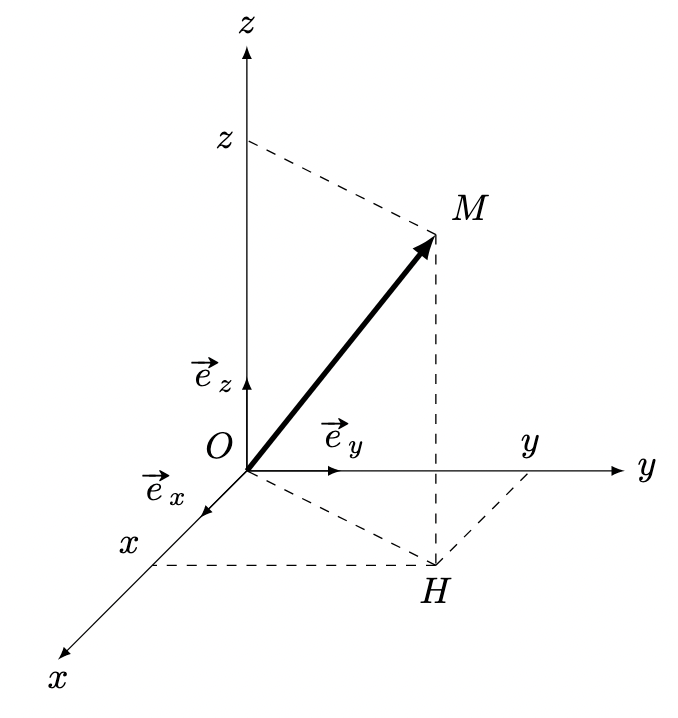
\includegraphics[width=5.2cm]{Figures/cartesien.png}&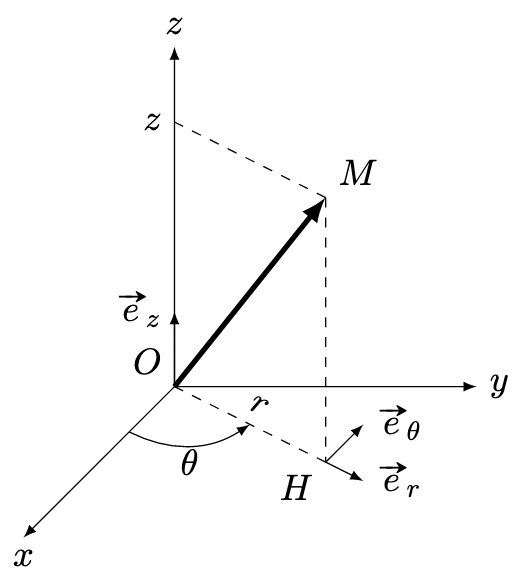
\includegraphics[width=5.2cm]{Figures/cylin.png}&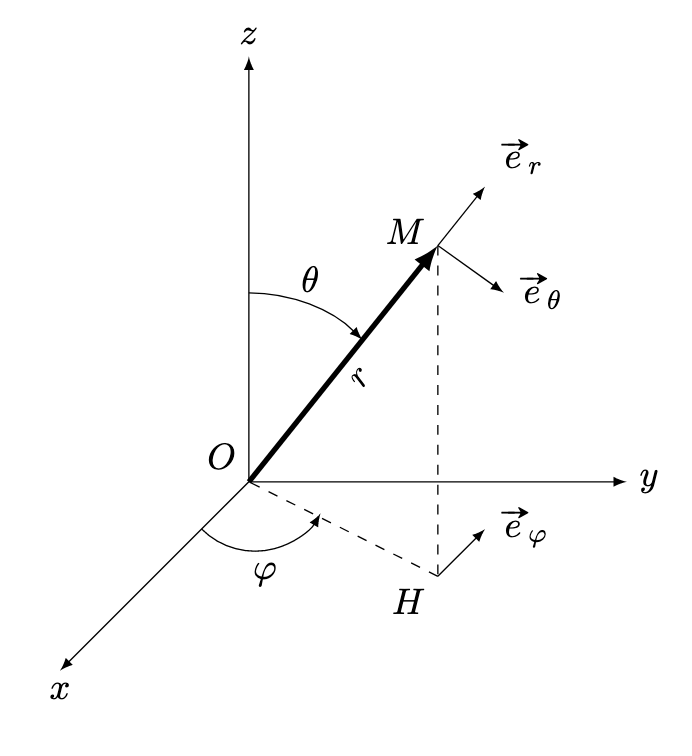
\includegraphics[width=5.2cm]{Figures/sphere.png}\\ \hline
        \multirow{2}{*}{$\overrightarrow{OM}$}&\multirow{2}{*}{$x\vec e_x+y\vec e_y+z\vec e_z$} &\multirow{2}{*}{$r\vec e_r+z\vec e_z$}&\multirow{2}{*}{$r\vec e_r$}\\
        &&&
        \\ \hline
        \multirow{2}{*}{$d\overrightarrow{OM}$}&\multirow{2}{*}{$d x\vec e_x+d y\vec e_y+d z\vec e_z$}&\multirow{2}{*}{$d r\vec e_r+r d \theta\vec e_\theta+d z\vec e_z$}&\multirow{2}{*}{$d r\vec e_r+rd \theta\vec e_\theta+r\sin\theta d \varphi \vec e_\varphi$}\\
        &&&
        \\ \hline
        \multirow{2}{*}{$\overrightarrow{v}$}&\multirow{2}{*}{$\dot x\vec e_x+\dot y\vec e_y+\dot z\vec e_z$}&\multirow{2}{*}{$\dot r \vec e_r+r\dot \theta \vec e_\theta+\dot z\vec e_z$}&\multirow{2}{*}{$\dot r\vec e_r+r\dot \theta\vec e_\theta+r\sin\theta\dot \varphi \vec e_\varphi$}\\
        &&&
        \\ \hline


        \end{tabular}
        \end{adjustwidth}
        \end{center}
        \label{default}
        \end{table}%


        \vspace{-0.7  cm}

        \textbf{Remarque} : Vous devez également savoir établir l'expression du vecteur accélération $\vec a$ dans le cas des coordonnées cartésiennes et cylindriques. Pour cela on retiendra surtout qu'avec les coordonnées cylindriques : \[\fbox{$\dfrac{d \vec e_r}{d t}=\dot \theta \vec e_\theta$} \hspace{1cm} \mathrm{et} \hspace{1cm} \fbox{$\dfrac{d \vec e_\theta}{d t}=-\dot \theta \vec e_r$}\]
    
\newpage
%%%%%%%%%%%%%%%%%%%%%%%%%%%%%%%%%%%%%%%%%%%%%%%%%%%%%%%%%%
\section{Lois de Newton}
\vspace{3cm}
    \subsection{Quantité de mouvement}
        \begin{DashedDefinition}{}[
            \begin{itemize}
                \item \textbf{Quantité de mouvement:} \[\vec p (M)_{/R}=m \vec v (M)_{/R}\]
                \item \textbf{Centre de masse:} \[m \overrightarrow{OG}=\sum_{k=1}^N m_k \overrightarrow{OM}_k\]
            \end{itemize}
        \end{DashedDefinition}
    \subsection{Lois de Newton}
        \begin{DashedDefinition}{}[
            \begin{itemize}
                \item \textbf{1er principe:} tout corps conservera son état de repos ou de mouvement uniforme en ligne droite dans lequel il se trouve, à moins qu'une force ne soit appliquée sur ce corps. (Principe vérifié pour un repère galiléen).
                \item \textbf{2eme principe} (PFD): \[\fbox{$\sum_i \overrightarrow{F}_{ext \rightarrow M,i} = m \vec a$}\]
                \item \textbf{3eme principe} (Actions réciproques): \[\overrightarrow{F}_{A \rightarrow B} = - \overrightarrow{F}_{B \rightarrow A}\]
            \end{itemize}
        \end{DashedDefinition}
        
    \subsection{Forces de frottements quadratiques}
        \begin{DashedDefinition}{}[
            Solide en mouvement dans un fluide à une vitesse importante $\overrightarrow{v}$, la force de frottements est $\overrightarrow{f}$:
            \[\overrightarrow{f}=-\beta ||\overrightarrow{v}|| \overrightarrow{v}\]
            * Avec $\beta$ le \textbf{coefficient de frottement}. \\
            Unité SI: \textbf{$kg.s^{-1}$} \\
            \textit{Voir page 11, pour les frottements linéaires.}
        \end{DashedDefinition}

\newpage
%%%%%%%%%%%%%%%%%%%%%%%%%%%%%%%%%%%%%%%%%%%%%%%%%%%%%%%%%%
\section{Approche énergétique du mouvement d'un point}
\vspace{3cm}
    \subsection{Puissance et travail}
        \subsubsection{Puissance}
            \begin{DashedDefinition}{}[
                La \textbf{puissance} d'une force $\vec F$, appliquée au point matériel M, d'une vitesse $\vec v$, dans le référentiel \( \mathcal{R} \):
                \[ \mathcal{P}(\vec F)_R=\vec F \cdot \vec v (M)_R\]
                USI: W(Watt)
            \end{DashedDefinition}
        \subsubsection{Travail}
            \begin{DashedDefinition}{}[
            \begin{itemize}
                \item \textbf{Travail élémentaire:} $\delta W (\vec F)_R = P(\vec F)_R dt = \vec F \cdot d \overrightarrow{OM}$
                \item \textbf{Travail entre $t_1$ et $t_2$:} \[W_{M_1 \rightarrow M_2}(\vec F)_R=\int_{M_1}^{M_2} \delta W(\vec F)_R=\int_{M_1}^{M_2} = F \cdot d \overrightarrow{OM}\]
            \end{itemize}
            USI: Joule (J)
            \end{DashedDefinition}
    \subsection{Théorèmes énergétiques}
        \subsubsection{Théorème de de la puissance et de l'énergie cinétiques}
            \begin{DashedDefinition}{}[
                \begin{itemize}
                    \item \textbf{Puissance cinétique:}
                    \[\frac{dE_c}{dt} = \sum_i P( \vec F_i)\]
                    \item \textbf{Énergie cinétique:}
                    \[\Delta E_c = \sum_i W_{M_1 \rightarrow M_2}(\vec F_1)=E_c(t_2)-E_c(t_1)\]
                    \textit{$M_1$ (resp. $M_2$) aux instants $t_1$ (resp. $t_2$)}
                \end{itemize}
            \end{DashedDefinition}
        \subsubsection{Théorème de de la puissance et de l'énergie mécaniques}
        \begin{DashedDefinition}{}[
            \begin{itemize}
                \item \textbf{Puissance mécanique:}
                \[\frac{dE_m}{dt}=\sum P(\vec F_{nc})\]
                Avec $P_{nc}$ la puissance des forces non conservatives: $P(\vec F_{nc})=\vec F_{nc} \cdot \vec v$
                \item \textbf{Énergie mécanique:}
                \[\Delta E_m(M)= \sum_k W_{M_1 \rightarrow M_2}(\vec F_{nc,k})=W_{nc}\]
            \end{itemize}
        \end{DashedDefinition}

    \subsection{Énergie potentielle}
        \begin{DashedDefinition}{}[
            Si une force est conservative (\textbf{indépendant du chemin suivi}), on a 
            \[\delta W (\vec F) = \vec F \cdot d \overrightarrow{OM} = -d E_p\]
        \end{DashedDefinition}
        L'énergie potentielle $E_p$ d'une force conservative $\vec F$ est: \fbox{$\vec F = - \overrightarrow{grad} E_p$}

    \subsection{Énergie mécanique}
        \begin{DashedDefinition}{}[
            L'énergie potentielle $E_p$ du point M correspond à la somme des énergies potentielles associées aux forces conservatives. L'énergie mécanique $E_m$ du point M est:
            \[E_m(M)=E_c(M)+E_p(M)\]
        \end{DashedDefinition}
\newpage
%%%%%%%%%%%%%%%%%%%%%%%%%%%%%%%%%%%%%%%%%%%%%%%%%%%%%%%%%%
\section{Mouvement de particules chargées}
\vspace{2cm}
 dans des champs électriques et magnétiques uniformes et stationnaires.  \\

    \subsection{Force de Lorentz}
    \begin{DashedDefinition}{}[
        Une particule chargée de charge $q$, animée d'une vitesse $\vec v$ dans un référentiel $\mathcal{R}$ subit, en présence d'un champ électrique $\vec E$ et d'un champ mangnétique $\vec B$, la force de Lorentz dont l'expression est:
        \[\fbox{$\vec F = q(\vec E + \vec v \wedge \vec B)$}\]
        On a aussi: $\vec F_m = q \vec v \wedge \vec B$ la force magnétique et est orthogonale à $\vec v$; \\ et $\vec F_e$ la force électrique.
    \end{DashedDefinition}
    \begin{itemize}
        \item La \textbf{force magnétique} est orthogonale à la vitesse, la puissance et le travail sont nuls. Elle \textbf{ne peut pas dévier} la particule chargée.
        \item La \textbf{force électrique} peut délivrer une puissance à une particule chargée. Elle peut \textbf{agir sur la norme et la direction} de la particule chargée.
    \end{itemize}

    \subsection{Mouvement dans un champ électrostatique uniforme}
        Le vecteur accélération est \textbf{constant}
        \begin{DashedDefinition}{}[
            Potentiel électrostatique (V): \fbox{$\vec E = - \overrightarrow{grad} V$} \\
            On a donc l'énergie potentiel: $E_p = qV$
        \end{DashedDefinition}
\newpage
%%%%%%%%%%%%%%%%%%%%%%%%%%%%%%%%%%%%%%%%%%%%%%%%%%%%%%%%%%
\section{Loi du moment cinétique du point}
\vspace{3cm}

    \subsection{Moment cinétique}
        \subsubsection{Moment cinétique par rapport à un point}
        \begin{DashedDefinition}{}[
            Un point M de masse m et de vitesse $\vec v$, dans un référentiel $\mathcal{R}$. Le \textbf{moment cinétique du point M par rapport au point A} dans le référentiel $\mathcal{R}$ est:
            \[\vec L_A(M)=\overrightarrow{AM} \wedge \vec p (M) = m \overrightarrow{AM} \wedge \vec v (M)_R\]
            USI: $kg \cdot m^{-1} \cdot s^{-1}$
        \end{DashedDefinition}

        \subsubsection{Moment cinétique par rapport à un axe $\Delta$}
        \begin{DashedDefinition}{}[
            Soit ($\Delta$) un axe orienté par un vecteur unitaire $\vec u_\Delta$ et A un point de cet axe. Le \textbf{moment cinétique} $L_\Delta(M)$ de M dans $\mathcal{R}$ par rapport à ($\Delta$) est le projeté orthogonal de $\vec L_A(M)$ sur ($\Delta$):
            \[L_\Delta(M)_R = \vec L_A(M)_R \cdot \vec u_\delta\]
        \end{DashedDefinition}
        
    \subsection{Moment d'une force}
        \subsubsection{Moment d'une force par rapport à un point}
            \begin{DashedDefinition}{}[
            Il s'agit de:
            \[\overrightarrow{\mathcal{M}_A}(\vec F)= \overrightarrow{AM} \wedge \vec F\]
            USI: N.m
            \end{DashedDefinition}
            
        \subsubsection{Moment d'une force par rapport à un axe $\Delta$}
            \begin{DashedDefinition}{}[
            Il s'agit de:
            \[\mathcal{M}_\Delta(\vec F)= \mathcal{M}_A(\vec F) \cdot \vec u_\Delta\]
            \end{DashedDefinition}
            
    \subsection{Loi du moment cinétique (LMC)}
        \subsubsection{LMC par rapport à un point fixe}
            \begin{DashedDefinition}{}[
                Soit un point matériel M de masse m mobile dans un référentiel \textbf{galiléen}. Soit un point A \textbf{fixe} dans $\mathcal{R}$.
                \[\frac{d \vec L_A(M)}{dt}=\sum_i \overrightarrow{\mathcal{M}_A}(\vec F_i)=\overrightarrow{\mathcal{M}_A} (\sum_i F_i)\]
            \end{DashedDefinition}
            
        \subsubsection{LMC par rapport à un axe fixe}
            \begin{DashedDefinition}{}[
                Soit un point maétriel M de masse m mobile dans un référentiel \textbf{galiléen}. Soit un axe $\Delta$ \textbf{fixe} dans $\mathcal{R}$.
                \[\frac{dL_\Delta(M)}{dt}=\sum_i \mathcal{M}_\Delta(\vec F_i)= \mathcal{M}_\Delta \cdot \sum_i(\vec F_i)\]
            \end{DashedDefinition}

\newpage
%%%%%%%%%%%%%%%%%%%%%%%%%%%%%%%%%%%%%%%%%%%%%%%%%%%%%%%%%%
\section{Mouvements dans un champ de force centrale conservatif}
\vspace{3cm}

    \subsection{Force centrale}
        \begin{DashedDefinition}{}[
            Une force $\vec F$ s'appliquant au point M est dite de \textbf{centrale de centre O} si quelle que soit la position de M, $\vec F$ est dirigée selon $\overrightarrow{OM}$
        \end{DashedDefinition}
        \textbf{Exemples:}
        \begin{table}[h!]
            \centering
            \begin{tabular}{c|c|c|c|c}
            Force & gravitationnelle & électrostatique & élastique & frottement fluide \\\hline
            & $\vec F_{O/M}= -G \frac{m_0 m\overrightarrow{OM}}{\overrightarrow{OM}^3}$ & $\vec F_{q_0/q_p}= \frac{1}{4 \pi \epsilon_0} \frac{q_0 q\overrightarrow{OM}}{\overrightarrow{OM}^3}$ & $\vec F_{el}=-k(r-l_0)\vec u_r$ & $\vec f = -h \dot{r} \vec u_r$
            \end{tabular}
        \end{table}
        \textit{Si un point M est soumis à une force centrale alors} $\vec L_0(M)$ \textit{est} \textbf{constante} \\
        Le mouvement à force force centrale est don \textbf{plan}.

        \subsubsection{Loi des aires}
            \begin{DashedDefinition}{}[
                \begin{itemize}
                    \item Pour un mouvement à force force centrale dans le plan en coordonées polaires, l'origine le centre de la force, on définit la \textbf{constante des aires}:
                    \[C=r^2 \dot{\theta}\]
                    USI: $m^2 \cdot s^{-1}$
                    \item Les \textbf{aires balayées} par le rayon vecteur pendant des intervalles \textbf{de temps égaux} $\Delta t$ valent:
                    \[\Delta \mathcal{A} = \frac{1}{2} C \Delta t\]
                \end{itemize}
            \end{DashedDefinition}
            
     \subsection{Force central conservative}
        Soit $\vec F$ une force centrale, elle est conservative si \fbox{$\vec F = - \overrightarrow{grad} E_p$}. Soit:
        \begin{DashedDefinition}{}[
            Une \textbf{force centrale conservative} et son énergie potentielle ne dépendent que de la première coordonnée sphérique ($|| \overrightarrow{OM} ||$) $r$ du point $M$:
            \[\vec F = F(r) \vec u_r = - \frac{dE_p}{dr} \vec u_r\]
        \end{DashedDefinition}
        \textbf{Exemples:}
        \begin{table}[h!]
            \centering
            \begin{tabular}{c|c|c|c}
            Force & gravitationnelle & électrostatique & élastique \\\hline
            & $E_p= -G \frac{m_0 m}{r}+cte$ & $E_p= \frac{q_0 q}{4 \pi \epsilon_0} + cte$ & $E_p= \frac{1}{2} k(r-l_0)^2 +cte$
            \end{tabular}
        \end{table}

        \subsubsection{Conservation de l'énergie mécanique et énergie potentielle effective}
            \begin{DashedDefinition}{}[
                L'énergie mécanique est \textbf{invariant du mouvement}:
                \[Em=\frac{1}{2}m \dot{r}^2 + \frac{1}{2} m \frac{C^2}{r2} + E_p(r)\]
                On définit \textbf{l'énergie potentielle effective} comme étant la somme des énergie cinétique orthoradial et potentielle:
                \[E_{pff}=\frac{1}{2} m \frac{C^2}{r^2} + E_p(r)\]
                \textit{Tout se passe comme si le système ne dépendait que d'une seule variable r}.
            \end{DashedDefinition}

    \subsection{Champs newtoniens}
        \begin{DashedDefinition}{}[
            Une force centrale \textbf{newtonienne} est de la forme \fbox{$\vec F = - \frac{K}{r^2} \vec u_r$}, avec K une constante.
            \begin{itemize}
                \item attractive si $K>0$
                \item répulsive si $K<0$
            \end{itemize}
        \end{DashedDefinition}

        \subsubsection{Lois de Kepler}
            \begin{DashedDefinition}{}[
                \begin{itemize}
                    \item 1er loi: Les planètes du système solaire décrivent des trajectoires elliptiques dont le Soleil occupe l'un des foyers
                    \item 2ème loi (Loi des aires): Le rayon vecteur Soleil-planète $\overrightarrow{SP}$ balaie des aires égales pendant des intervalles de temps égaux.
                    \item 3ème loi: La période de révolution T et le demi-grand axe $a$ de l'ellipse sont tels que $\frac{T^2}{a^3}$ a la même valeur pour toutes les planètes du système solaire.
                \end{itemize}
            \end{DashedDefinition}
\newpage
%%%%%%%%%%%%%%%%%%%%%%%%%%%%%%%%%%%%%%%%%%%%%%%%%%%%%%%%%%
\section{Mouvement d'un solide}
\vspace{3cm}
    Un solide est un système matériel \textbf{indéformable}. La distance entre les points matériels reste constante.
    \subsection{Théorème du moment cinétique autour d'un axe}
        \subsubsection{Moment cinétique}
            Soit $\Delta$ un axe orienté fixe et S un solide en rotation autour de cet axe, le solide S modélisé par un ensemble de point $M_k$. Le moment cinétique du solide par rapport à l'axe est:
            \[\fbox{$L_\Delta = \sum_k L_\Delta(M_k)$}\]
        \subsubsection{Moment d'inertie}
            \begin{DashedDefinition}{}[
                Le \textbf{moment d'inertie} du solide S par rapport à l'axe $\Delta$ est:
                \[\sum_k m_k r_k^2\]
                \textit{Avec $r_k$ la distance entre le point $M_k$ et l'axe} \\
                Le \textbf{moment cinétique} d'un solide en rotation à vitesse $\omega$ autour d'un axe fixe ($\Delta$)\textbf{orienté} par le vecteur unitaire $\vec u_\Delta$ est:
                \[L_\Delta(S)= J_\Delta \omega\]
            \end{DashedDefinition}
        \subsubsection{Moment d'une force}
            \begin{DashedDefinition}{}[
                Pour un solide S, le moment d'une force $\vec F$, subie par le point $M_k$ (point d'application de la force) par rapport à l'axe orienté $\Delta$ est:
                \[\mathcal{M}_\Delta(\vec F)=(\overrightarrow{AM_k} \wedge \vec F) \cdot \vec u_\Delta\]
            \end{DashedDefinition}
        \subsubsection{Liaison pivot}
            L'action mécanique d'une liaison pivot parfaite a un moment nul:
            \[\mathcal{M}_{\Delta (laison idéale)}=0\]
        \subsubsection{Théorème scalaire du moment cinétique}
            \begin{DashedDefinition}{}[
                Mouvement d'un solide S en rotation autour de $`\Delta$ fixe dans un référentiel galiléen, moment d'inertie $J_\Delta$, vitesse angulaire $\omega = \dot{\theta}.$
                \[\frac{dL_\Delta}{dt} = J_\Delta \frac{d \omega}{dt} = \mathcal{M}_\Delta^{ext}\]
            \end{DashedDefinition}
    \subsection{Approche énergétique}
        L'\textbf{énergie cinétique} d'un solide S en rotation s'écrit:
        \[E_c(S)=\frac{1}{2} J_\Delta \dot{\theta}^2 = \frac{1}{2} J_\Delta \omega^2\]
        \subsubsection{Puissance et travail}
        \begin{DashedDefinition}{}[
            La \textbf{puissance} d'une Force $\vec F$ en $M_k$ d'un solide S est:
            \[\mathcal{P}(\vec F)=\vec F \cdot \vec v_k\]
            Dans le cas où le solide est en rotation autour de $\Delta$:
            \[\mathcal{P}(\vec F)=\mathcal{M}_\Delta(\vec F)\omega\]
            Le \textbf{travail} est:
            \[\delta W(\vec F)= \vec F \cdot d \overrightarrow{OM}_k = P(\vec F)dt\]
        \end{DashedDefinition}
        \subsubsection{Théorèmes énergétiques}
            \begin{DashedDefinition}{}[
            Soit S un \textbf{solide indéformable}. \\
            \textbf{Théorème de l'énergie cinétique}:
            \[\Delta E_c(S) = W^{ext}\]
            \textbf{Théorème de la puissance cinétique}:
            \[ \frac{d E_c(S)}{dt} = \mathcal{P}^{ext}\]
            Avec $\mathcal{P}^{ext} = \mathcal{M}_\Delta^{ext} \omega$
            \end{DashedDefinition}
\newpage
%%%%%%%%%%%%%%%%%%%%%%%%%%%%%%%%%%%%%%%%%%%%%%%%%%%%%%%%%%
%\section{Système thermodynamique à l'équilibre}
%\vspace{3cm}
%    {\huge LA PARTIE THERMO SERA FAIT EN MÊME TEMPS QUE LES FICHES DE DEUXIÈME ANNÉE}
%\newpage
%%%%%%%%%%%%%%%%%%%%%%%%%%%%%%%%%%%%%%%%%%%%%%%%%%%%%%%%%%
%\section{Échange et bilan d'énergie, 1er principe}
%\vspace{3cm}
%    {\huge LA PARTIE THERMO SERA FAIT EN MÊME TEMPS QUE LES FICHES DE DEUXIÈME ANNÉE}
%\newpage
%%%%%%%%%%%%%%%%%%%%%%%%%%%%%%%%%%%%%%%%%%%%%%%%%%%%%%%%%%
%\section{Second principe et bilan entropique}
%\vspace{3cm}
%    {\huge LA PARTIE THERMO SERA FAIT EN MÊME TEMPS QUE LES FICHES DE DEUXIÈME ANNÉE}
%\newpage
%%%%%%%%%%%%%%%%%%%%%%%%%%%%%%%%%%%%%%%%%%%%%%%%%%%%%%%%%%
%\section{Étude des machines thermiques}
%\vspace{3cm}
%    {\huge LA PARTIE THERMO SERA FAIT EN MÊME TEMPS QUE LES FICHES DE DEUXIÈME ANNÉE}
%\newpage
%%%%%%%%%%%%%%%%%%%%%%%%%%%%%%%%%%%%%%%%%%%%%%%%%%%%%%%%%%
\section{Champ magnétiques - description}
\vspace{3cm}
    Un \textbf{champ magnétique}, noté $\vec B(M,t)$ est un \textbf{champ vectoriel}. USI: Tesla(T).
    \subsection{Cartes de champ magnétiques}
    \begin{DashedDefinition}{}[
        \begin{itemize}
            \item Une \textbf{ligne de champ} est une courbe \textbf{tangente au champ magnétique} en chacun de ces points et \textbf{orientée} dans le sens du camp.
            \item Un \textbf{spectre de champ} est un ensemble de lignes de champ magnétique.
        \end{itemize}
    \end{DashedDefinition}
        \begin{itemize}
            \item Les lignes de champs (l.d.c) sortent par le pôle nord et entrent par le pôle sud à l'extérieur de la source.
            \item Le champ est plus intense dans les zones où les l.d.c se rapprochent.
            \item Les l.d.c parallèles révèlent d'un champ uniforme.
        \end{itemize}
    \subsection{Moment magnétique}
        \begin{DashedDefinition}{}[
            Soit un circuit filiforme plan constitué d'un boucle parcourue par un courant I. Le moment magnétique $\overrightarrow{\mathcal{M}}$ en (A.m²) du circuit est défini par:
            \[\fbox{$\overrightarrow{\mathcal{M}}=i \vec S$}\]
            où $\vec S = S \vec n$ le vecteur surface de norme S et de normal $\vec n$, \textbf{orthogonal} au plan contenant le circuit, et \textbf{orienté} par le sens du courant.
        \end{DashedDefinition}

\newpage
%%%%%%%%%%%%%%%%%%%%%%%%%%%%%%%%%%%%%%%%%%%%%%%%%%%%%%%%%%
\section{Action d'un champ magnétiques}
\vspace{3cm}
    \subsection{Force de Laplace}
    \begin{DashedDefinition}{}[
        Dans le cas d'une barre conductrice MN placée dans un champ magnétique extérieur uniforme $\vec B$ parcouru par un courant d'intensité $i$ et stationnaire, l'expression de la \textbf{résultante des forces de Laplace} est:
        \[\vec F_L = \int_M^N i \vec{dl} \wedge \vec B = \fbox{$i \overrightarrow{MN} \wedge \vec B$}\]
        \textbf{Le vecteur $\overrightarrow{MN}$ est orienté par la convention choisie pour le courant $i$} \\
        La \textbf{puissance} vaut:
        \[P_l=(i\overrightarrow{MN} \wedge \vec B) \cdot \vec v\]
    \end{DashedDefinition}

    \subsection{Moment du couple de Laplace}
        \begin{DashedDefinition}{}[
            Soit une spire \textbf{rectangulaire} en rotation autour de $Oz$, axe de symétrie, placé dans un champ magnétique extérieur uniforme et stationnaire orthogonal $Oz$.
            \begin{itemize}
                \item La résultante des forces de Laplace exercée sur la spire est nulle.
                \item Le couple des actions de Laplace vaut:
                \[ \fbox{$ \vec \Gamma = \overrightarrow{\mathcal{M}} \wedge \vec B $ }\]
                Avec $\overrightarrow{\mathcal{B}}$ le vecteur magnétique de la spire rectangulaire.
                \item La puissance tournant à une vitesse \textbf{angulaire $\omega$} autour de ($Oz$):
                \[P= \Gamma \cdot \omega = \omega (\overrightarrow{\mathcal{M}} \wedge \vec B)\cdot \vec u_z\]
            \end{itemize}
        \end{DashedDefinition}
        Le couple des actions mécaniques tend à orienter le moment magnétique d'un aimant, selon la direction de $\vec B$.
\newpage
%%%%%%%%%%%%%%%%%%%%%%%%%%%%%%%%%%%%%%%%%%%%%%%%%%%%%%%%%%
\section{Circuit fixe dans un champ magnétique}
\vspace{3cm}
    \subsection{Lois de l'induction}
        \subsubsection{Flux magnétique}
        \begin{DashedDefinition}{}[
        \begin{wrapfigure}{r}{0.25\textwidth}
            \centering
            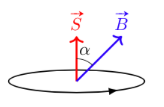
\includegraphics[width=0.25\textwidth]{Figures/Induction1.png}
        \end{wrapfigure}
        Soit une surface plane (S), de normale $\vec n$, fixe sur un contour orienté (règle de la main droite) et un champ magnétique \textbf{uniforme} traversant cet surface dépendant du temps $\vec B(t)$. Le flux magnétique est:
        \[\Phi (t) = \vec B(t) \cdot \vec S = \vec B(t) \cdot \vec n S=BScos(\vec B, \vec S)\]
        USI: Weber (Wb). \\
        Le flux de $\vec B$ uniforme à travers une bobine de N spires de même surface S est: $\Phi = N \vec B \cdot \vec n S$
        \end{DashedDefinition}

        \subsubsection{Loi de Lenz-Faraday}
        \begin{DashedDefinition}{}[
            La \textbf{force électromotrice}, $e$ (en Volt; V), induite par le champ magnétique $\vec B$ dans un \textbf{circuit} élecrique filiforme fermé et \textbf{orienté arbitraiement} est:
            \[e(t)=- \frac{d \Phi(t)}{dt}\]
        \end{DashedDefinition}

        \subsubsection{Loi de modération de Lenz}
        \begin{DashedDefinition}{}[
        \textbf{Par leurs effets, les phénomènes d'induction s'opposent aux causes qui leur ont donné naissance.}
        \end{DashedDefinition}
        \textit{Le circuit peut se déformer ou se déplacer en présence d'un champ magnétique permanent ; c'est l'induction de Lorentz. L'inducteur peut produire un champ magnétique variable à travers un circuit fixe c'est l'induction de Neumann.}

        \subsection{Phénomène d'auto induction}
            \subsubsection{Flux propre et inductance propre}
                \begin{DashedDefinition}{}[
                On considère un circuit parcouru par un courant $i$.  Le champ magnétique $\vec B_p$ crée est le \textbf{champ propre}. Le propre est le flux de $B_p$ à travers une surface S, noté $\Phi_p$. Soit:
                \[L=\frac{\Phi_p}{i}\]
                L est une constante nommée inductance propre en Henry.
                \end{DashedDefinition}
            \subsubsection{Force électromotrice (f.é.m) induite}
                \begin{DashedDefinition}{}[
                Lorsque le courant $i(t)$ dans un circuit fixe et indéformable est variable, le flux propre varie. Il s'agit de \textbf{l'auto-induction.}
                \[e=-\frac{d \Phi_p}{dt} = -\frac{dLi}{dt} = -L \frac{di}{dt}\]
                \end{DashedDefinition}
            \subsection{Approche énergetique}
                \begin{DashedDefinition}{}[
                L'\textbf{énergie magnétique} stockée grâce aux phénomènes d'auto-induction dans un circuit d'inductance propre L parcourue par un courant $i$ est égale à: $\frac{1}{2} L i^2$
                \end{DashedDefinition}

        \subsection{Induction mutuelle}
            \begin{DashedDefinition}{}[
             Le \textbf{flux mutuel} est le flux générée par un circuit inducteur sur le circuit induit.
             \[\Phi_{1 \rightarrow 2}(t)=M_{12}i_1(t); \Phi_{2 \rightarrow 1}(t)=M_{21}i_2(t)\]
             Théorème de Neumann: \fbox{$M_{12}=M_{21}=M$} \\
             Avec M, le coefficient d'inductance mutuelle en Henry (H).
            \end{DashedDefinition}
            On a: $E_{mag}=\frac{1}{2}L_1 i_1^2 + \frac{1}{2}L_2 i_2^2 + Mi_1i_2$ \\
            \textit{Avec $Mi_1i_2$ l'énergie de couplage magnétique entre les circuits.}
\newpage
%%%%%%%%%%%%%%%%%%%%%%%%%%%%%%%%%%%%%%%%%%%%%%%%%%%%%%%%%%
%\section{Circuit mobile dans un champ magnétique}
%\vspace{3cm}
%
%\newpage
%%%%%%%%%%%%%%%%%%%%%%%%%%%%%%%%%%%%%%%%%%%%%%%%%%%%%%%%%%%
\section{Lectures complémentaires}\label{sec:resources}
\vspace{3cm}
\textbf{Je fais plusieurs fois référence au Complément Mathématiques} ! \\
Merci à mes professeurs de physiques:
\begin{itemize}
    \item Emillien Mallet, pour les cours et la fourniture d'éléments en \LaTeX !
    \item Claire Delacour, pour les cours de deuxième année, une couche supplémentaire à la compréhension !
\end{itemize}


    \vfill
    \small{\noindent \textbf{Note:} \vspace{-3mm}\\
    \noindent \rule{3.3cm}{0.5pt} \\
        Venez en prépa !}
\newpage

%%%%%%%%%%%%%%%%%%%%%%%%%%%%%%%%%%%%%%%%%%%%%%%
%    \begin{thebibliography}{17}
%	\vspace{3.5cm}
%	\end{thebibliography}
%\addtocounter{section}{14}
%\addcontentsline{toc}{section}{\protect\numberline{\thesection}~~~ References}
%%%%%%%%%%%%%%%%%%%%%%%%%%%%%%%%%%%%%%%%%%%%%%%%%%%%%%%%%%%%%%%%%%
\end{document}